\section{Общее описание приложения}
\subsection{Используемые инструменты}

В разработке сайта был использован язык программирования Python и микрофреймворк Flask, который отвечал за обработку запросов клиента. Также в состав данного фреймворка входит шаблонизатор Jinja2.

Также использовался CSS-препроцессор - SASS. Он позволяет соблюдать принцип DRY (англ. Don't repeat yorself - не повторять свой код), предоставляя расширенные возможности, отсутствующие в CSS, а именно:
\begin{itemize}
	\item переменные - существует возможность один раз задать значение переменной, затем многократно использовать в коде;
	\item миксины - "функции" языка, сохранив целые части кода, можно использовать их многократно, в том числе с использованием переменных. Также существует ряд готовых библиотек (в данной работе использовалась библиотека Bourbon);
	\item вложенные стили и наследование - они позволяют использовать правила одного элемента в другом.
\end{itemize}

\subsection{Файловая структура приложения}
Файловая структура веб-приложения имеет следующий вид:

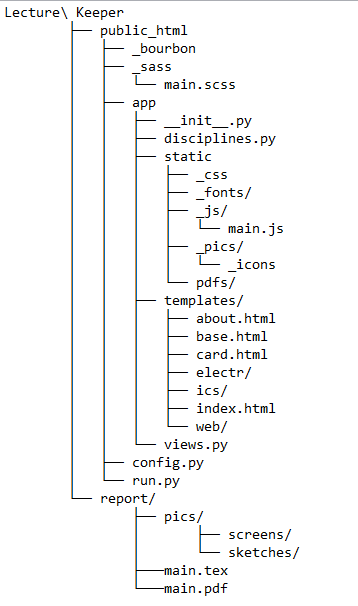
\includegraphics{codes/file_struct.png}

Запуск сервера осуществляется с помощью файла run.py:

\begin{lstlisting}
	python3 run.py
\end{lstlisting}

После запуска сервера приложения, оно становится доступно по адресу: http://localhost:5000. Для того, чтобы сделать сервер доступным в сети или включить режим отладки, необходимо внести следующие строки в файл config.py:

\begin{lstlisting}[language=Python]
	host=0.0.0.0
	debug=True
\end{lstlisting}

Каждая страница сайта формируется при запросе пользователя, шаблоны находятся по адресу /public\_html/app/templates/. Общий шаблон для всех страниц base.html отвечает за отображение панели навигации, бокового меню, контейнера с содержимым страницы и футера.

Главная страница сформирована из шаблона /public\_html/app/templates/index.html, в котором содержатся шаблоны "карточек дисциплин" равным количеству дисциплин, зарегистрированных в приложении.

Информация, для отображения страницы "About"\ находится в файле about.html. Тексты лекций находятся в соответствующих подкаталогах каталога /templates. Также существует возможность загрузки pdf-файла каждой лекции, которые находятся в директории /static. Также в этой папке находятся файлы, отвечающие за оформление страниц (/\_css/main.css) и за интерактивное поведение элементов страниц (/\_js/main.js). В каталоге /fonts расположены файлы гарнитур, используемые на страницах сайта.

В каталогах /\_sass и /bourbon находятся нескомпилированные файлы стилей и библиотека готовых стилей соответственно. 